%!TEX root = ../crimson_throne_book_main.tex
% 2016-02-20
\section{18 Arodus 4708}

The next morning, at breakfast, Sjo does not feel inclined to explore the city further. He fears that wandering about the city blindly and asking questions might raise more suspicion than answer questions. He trusts that the {\itshape Pinkhouse} is probably the best place to find the information he needs. Looking around the taproom he sees the same people who were here yesterday morning. The tall weapons dealer from Sandpoint is at one of the tables, as is Brugo, the cloth trader from Nimrathas, who is having a meal with his two men who look like his assistants. Puk, Quint and Balian visit the market with little Uri again, but do little more than stretch their legs. The most daring thing they do, is try a local specialty: bulette on a stick. After spending a couple of hours watching his pitcher of beer grow warm, Sjo sees the empty barroom fill up with a handful of customers again during lunchtime. Brugo returns, although he has left his assistants at the market. Sjo follows the trader to the toilet and starts a casual conversation. Brugo discreetly asks Sjo if he is a Shoanti, because the tribesmen from the Cinderlands are generally made to feel even less welcome in Urgir than other pinkskins. Sjo explains that he is a halfblood, but he still appreciates the warning. He wonders if Brugo knows about any remarkable incidents with Shoanti in the past. The trader says that he has heard some tales about Shoanti barbarians whose pride got in the way of \ldots surviving, and he adds that he actually knows of a Shoanti who lives here, but the man does his best not to look like one of the wildlings, in fact, he wears a clever disguise that makes him seem like a halforc. It's a daring, but sensible move, Brugo explains, especially for a man who does business in the all-orc districts. Brugo met him in {\itshape The Pit of Doom} , one of Urgir's fighting pits, where the man delivers monster for death matches. When his friends return, Sjo gets Uri to lead them to {\itshape The Pit} , but only after they have cast some long-term buffs, like  {\itshape heroism} . The orc boy proves his worth again by cleverly guiding the party through throngs of orcs, avoiding the meanest and toughest hotspots in the crowd. Using the hoods of their gray cloaks to hide their faces, Balian and Puk try to keep from being noticed, while Sjo and Quint imitate an orcish way of moving about to blend in. Uri keeps the pace high enough to prevent little mishaps. By the time a more perceptive orc suspects something fishy about the group, they have already moved on.  {\itshape The Pit of Doom} is situated in a part of the city that must have once been a warehouse district for the dwarves. The buildings here are bigger and more basic in design than the fancier neighborhoods the travelers have visited until now. Still, the orcs use most of these storehouses as apartment block in what feels like the run-down corner of town. One such barn-sized stone building bears a wooden sign above the entry, depicting a simple pit. The double doors stand ajar, allowing raucous laughter, curses and grunts to filter out to the street. Inside the depot serves as a massive taproom, with a ceiling that reaches a height of 20 feet. Thick stone arches support the slightly cracked roof and have chains hanging down from them with burning lanterns. The smell of cheap alcohol, blood and urine permeates the air, but does not seem to bother the many patrons, for indeed, despite the early hour, the place is already quite packed with orcs and a handful of half-orcs. The only humans in here are slaves who serve drinks and while none of them looks like fighters, they all bear signs of being beaten. The arrival of the gray cloaked party draws enough attention for one of the orc patrons to peek under Sjo's hood and recognize a pinkskin. The creature spits on the ground in front of the healer and growls: {\itshape``Hey, slave, fetch me a drink!}'' The others at his table burst into laughter, which makes even more orcs in the tavern aware of the company's presence. The heroes of Korvosa chose to ignore the provocation and pick a table at the far end of the room. The chairs have been nailed back together so many times that they look like the final failure of a dying one-handed carpenter with a blind eye. The whole bar is set up around a cave-in in  the center of the hall, which has been filled with earth to create a flat surface for the fighting pit. A stone pillar rises in the middle of the arena, heavy chains hanging from its sides. The bartender operates the place from a large caged bar at the back of the common room.\\

A human slave takes the party's order, eying them with a mixture of amazement and fear. His visit at the table is quickly followed by a burly orc who walks up with a broad smile of confidence on his scarred face. His hands rest casually on the pommels of two short swords, hanging from his belt. {\itshape``Tough pinkskin, come here looking for a fight, hey?}'' he spits in Orcish.\\

{\itshape``We heard about this wonderful place}'', Quint replies, weaving the power of fascination in his words, {\itshape``and the spectacular fights that it hosts. We wanted to see for ourselves, as spectators, of course.}'' Next the bard mixes a {\itshape suggestion} in his expos\'e: {\itshape``Why don't you get us a drink and tell us about it?}'' {\itshape``Har, har, I'll get you a drink all right, little man, while you think about who you're going to send into the pit to face me!}'' the orc shouts for the whole bar to hear. {\itshape``One versus one, or two versus two, your choice!}'' Next the orc does indeed get the companions some ale, expecting an answer to the challenge he issued upon his return. Sjo and Balian accept, having just learned from Uri that these death matches have no rules, so any magic is permitted. As the two of them descend into the arena, Puk joins the betting pool at the caged bar, matching all the orcs' money with 400 gold. The crowd gathers around the pit and starts shouting: {\itshape``Arrodok! Arrodok!}'' The orc gladiator jumps in as well and waits for his partner to arrive: a humongous troll with a hefty warhammer in his left hand and a cruel blade in his right. The onlookers purr with delight as the monster glides in the ring.\\

The troll is the first to strike: he lunges at Balian and glances the ranger's shoulder with his hammer. From the crowd Quint attempts to influence the fight with {\itshape satire} , but the loud cheers from the orcs around him drown his word of mockery. Arrodok and Balian exchange blows while Sjo surprises everyone by throwing two fireballs in rapid succession at his adversaries, having them wonder how the hell a fully-plated warrior casts spells like a wizard? Especially the troll seems shocked, obviously harboring a fathomless fear for fire. The flames of Sjo's fireball even blow over the edge of the pit, taking out three spectators in the crowd. Balian has a harder time impressing the bystanders and sees his swings parried. The troll has no doubts about who his biggest threat is and focuses his attention on Sjo. He rages with fury and knocks the fire-wielding warrior off his feet. Arrodok is likewise inspired and slices at Balian with swift strikes. Sjo, who is still on the ground, seeks to freeze the orc gladiator in place with a  {\itshape hold person} , but the fighter miraculously summons enough willpower to resist. Balian struggles to keep to his feet and counterattacks, cutting a deep gash in the orc with his first strike, but seeing his second blow go wide. Using heroic inspiration he attempts another hit, but threatens to miss again. From the side of the pit Quint interferes by having his bardic magic guide the ranger's attack true; the crowd's cries are so loud that they easily mask his meddling. Balian's corrected arch hits Arrodok hard in the head and the orc goes down. The troll grunts, but continues his furious charge on the prone fire-wielder and gets two more hits in. Sjo encloses the brute in a wall of fire, making the creature's morale drop even more. The troll's instincts tell him to run, his fear forcing him to give up his  {\itshape rage} and making him flee to the other side of the pit, where he takes a few breath to compose himself. Sjo uses the opportunity to get to his feet and cast a powerful  {\itshape cure critical wounds} on Balian, steering the ranger away from the edge of death. Balian now takes a defensive stand in front of Sjo, blocking the troll path to his friend. The troll is still a bit shaky on his feet, but rejoins the fight and tries to cut Balian out of his way to vengeance, but the ranger deflects almost all of his hits. In the meantime Sjo throws fireball upon fireball at the monster, until finally, he succumbs to the burns. The crowd around the pit suddenly goes quiet. Uri is the first to break the silence, as he yells out in victory and even urges the other orcs to applaud the companions' triumph as well, without success however. The shame of losing to pinkskins combined with the loss of money in the betting pool compels the patrons of the  {\itshape Pit of Doom} to muteness. While Sjo uses his powers of healing to patch him and Balian up, Quint and Puk head to the bar to pick up their winnings. Quint sees how the bartender reluctantly reaches for two pouches of coin. The bard inquires about the 'monsters' that are rumored to be an attraction in the pit, as he would love to see such beasts for himself. The barkeep says that he hasn't heard from his supplier in several days and when Quint prompts him to elaborate, he reveals that he normally buys his pit monsters from a half-orc named Hobar, who lives only two blocks away. His house is easy to spot, someone has painted a message on the barn door: {\itshape``Pinkskins out, orcs first!}'' Quint tips the orc and motions for his friends to leave.\\

Uri has no trouble locating Hobar's place, which has two points of entry: a big barn door and a set of double doors into the main building. Puk tries the lock and finds it open already.\hyperref[fig:Entering-Hobar-s-shop-591946639]{ He pushes in, stepping into a peculiar place of business, a monster dealership. }  \hyperref[fig:Hobar-s-monster-shop-in-Urgir-591945961]{ The room behind the counter houses two big cages: one with a dragon-like creature -- a mantidrake - and another one with three large birds. There is a wooden door behind the dragon cage and a set of stairs leading up. } Quint covers his friends in invisibility, but when they advance into the room, something behind the wooden door reacts to their presence. At that exact moment all doors open simultaneously, releasing the mantidrake and terror birds, and revealing two rust monsters behind door number three, their antennae feverishly reaching for the metal of the companions' arms and armor. \\

\begin{figure}[h]
	\centering
	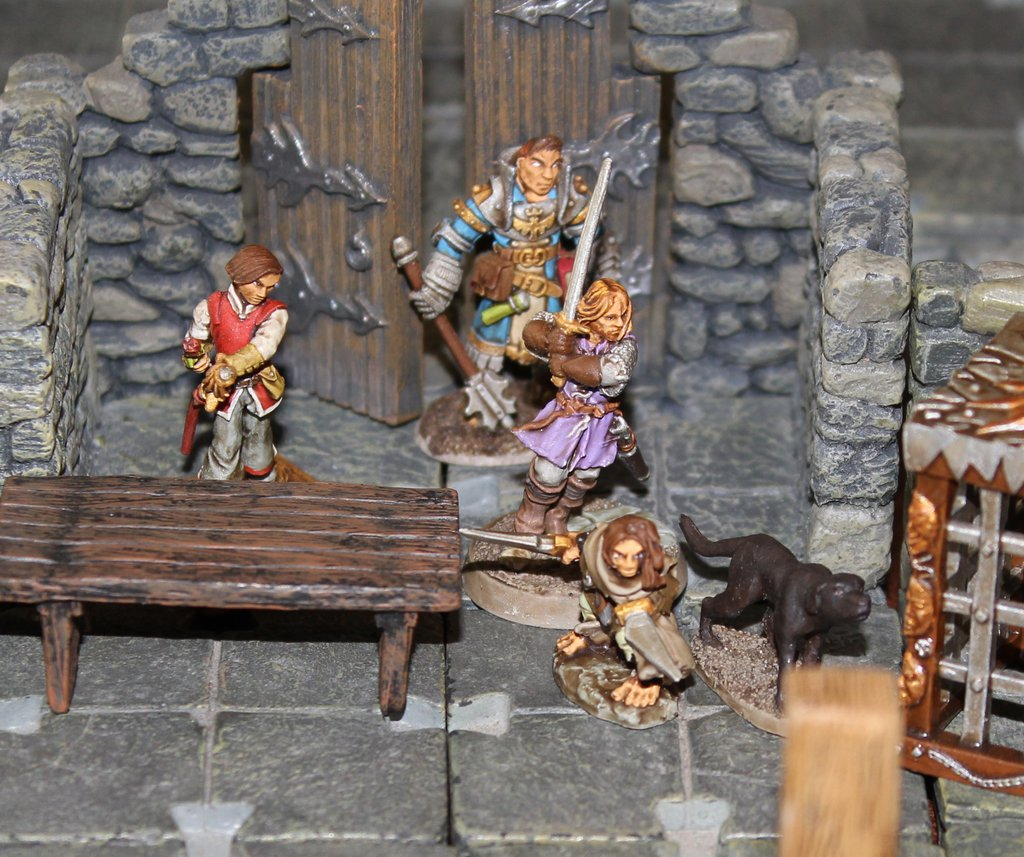
\includegraphics[width=0.39\textwidth]{images/Entering-Hobar-s-shop-591946639.jpg}
	\caption{Entering Hobar's shop}
	\label{fig:Entering-Hobar-s-shop-591946639}
\end{figure}

\begin{figure}[h]
	\centering
	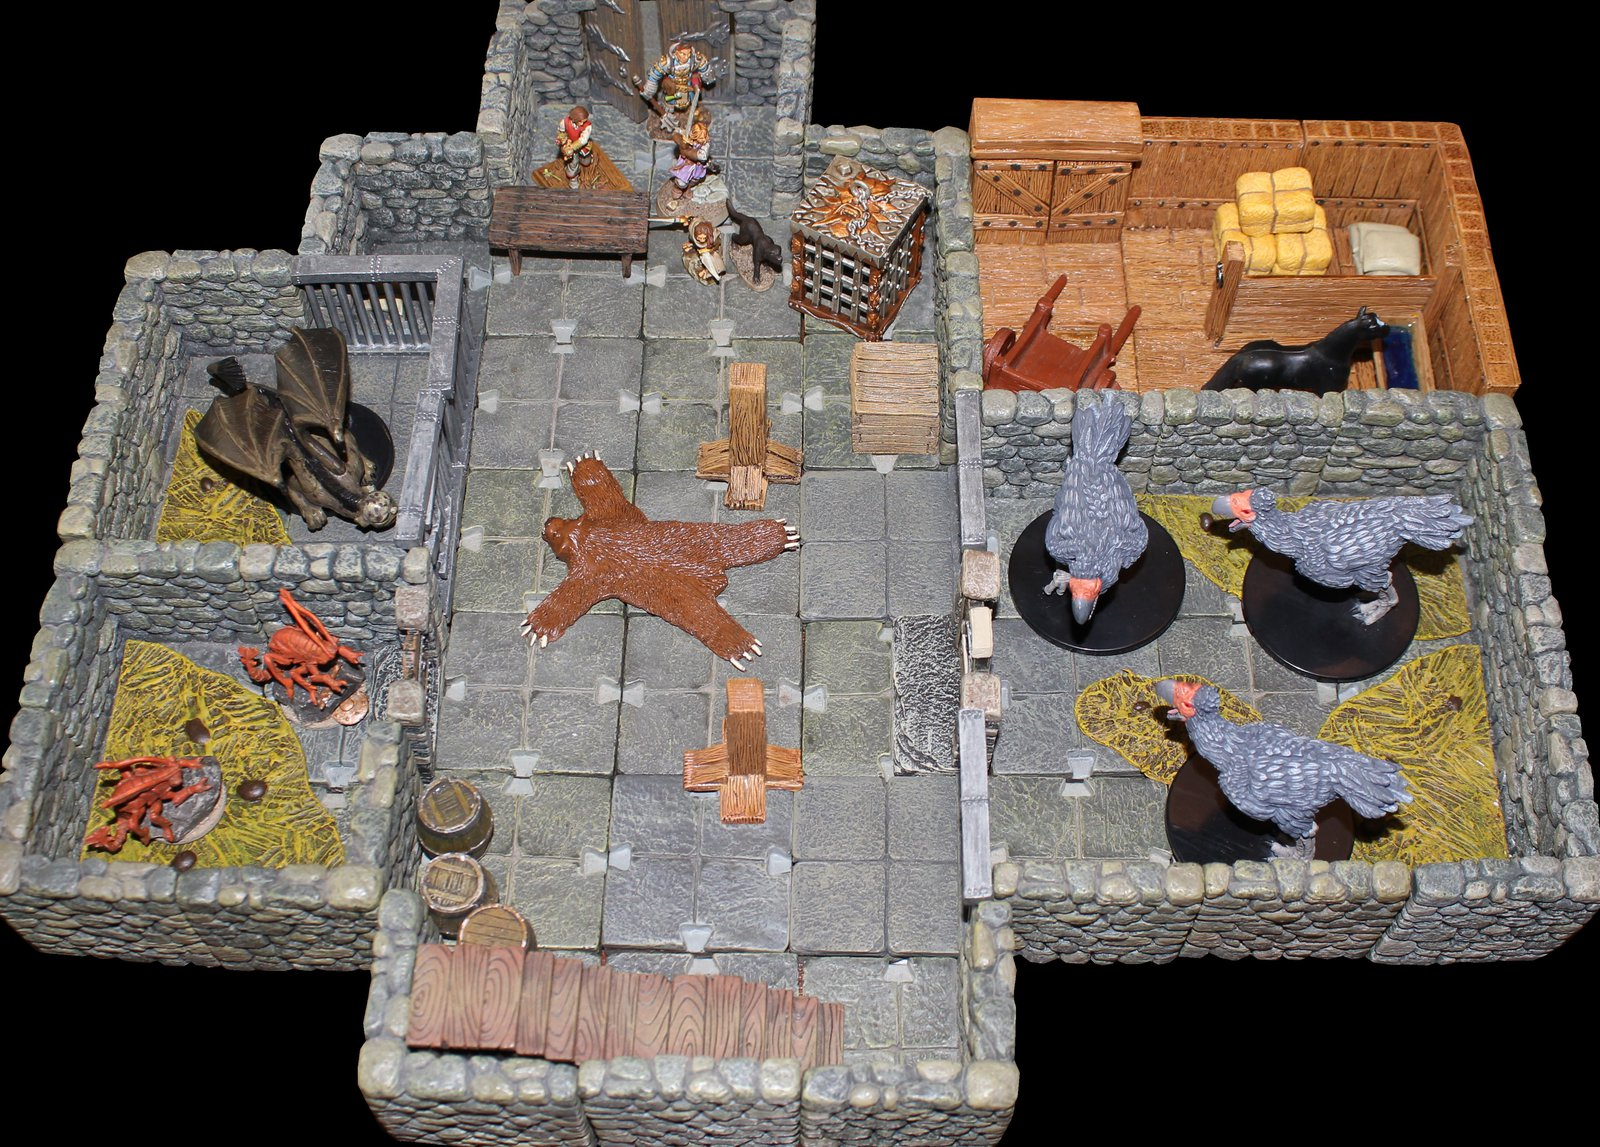
\includegraphics[width=0.39\textwidth]{images/Hobar-s-monster-shop-in-Urgir-591945961.jpg}
	\caption{Hobar's monster shop in Urgir}
	\label{fig:Hobar-s-monster-shop-in-Urgir-591945961}
\end{figure}

